% SC3010 --- Chapter 7: Operating System Security (0->100 ground-up)
% No \documentclass --- this file is \input/\include'd by main.tex.
\chapter{Operating System Security: Isolation and Containment}
\label{ch:os}
\begin{quote}
\emph{``The operating system is the reference monitor that never sleeps.''} --- Every application trusts the OS to keep its memory private, its files intact, and its privileges bounded. This chapter asks how that trust is built: by isolating, mediating, and containing.
\end{quote}
\noindent\fbox{\parbox{\dimexpr\linewidth-2\fboxsep-2\fboxrule}{%
\textbf{From zero: we build here, no OS course needed.} We assume you know what a process and a file are at an everyday level (a running program, a named blob of bytes). From that we build isolation, privilege, sandboxing, and virtualization from first principles---pictures before formalism, then definitions, examples, and analysis.}}
\vspace{0.4em}
\section*{Learning Outcomes}
After this chapter you will be able to:
\begin{enumerate}[label=(L\arabic*)]
    \item explain why isolation is the foundation of OS security and state the three reference-monitor properties;
    \item describe privilege separation, privilege bracketing, and the principle of least privilege with concrete mechanisms;
    \item compare sandboxing techniques (system-call filtering, capability-based, language-based);
    \item distinguish hypervisor types, VM isolation guarantees, and VM-escape threats;
    \item analyse container isolation (namespaces, cgroups, seccomp) and contrast containers with VMs.
\end{enumerate}
% ============================================================
\section{Why the OS Must Isolate}
\label{sec:os-why-isolate}
On a single machine dozens of programs run at once: your browser, a PDF reader opening an untrusted attachment, a background updater. Without isolation a bug in one becomes a compromise of all. Picture an apartment building: each flat has its own lock and walls; the hallway (kernel) mediates who may enter where.
Formally, \emph{isolation} means a fault or compromise in compartment $A$ cannot read, write, or control resources of compartment $B$ except through an explicit, mediated channel.
Two design principles follow immediately:
\begin{definition}[Least privilege \& complete mediation]
\emph{Least privilege:} every component holds only the privileges it needs to do its job, for the shortest time needed. \emph{Complete mediation:} every access to a protected resource is checked.
\end{definition}
Without least privilege a compromised renderer can read \texttt{/etc/shadow}; without complete mediation a check that can be bypassed is no check at all.
\begin{example}[Threat model without isolation]
Suppose the OS maps every process into the same physical address space with no MMU enforcement. A buffer overflow in the JPEG parser overwrites the banking app's memory and steals the session cookie. With per-process virtual address spaces and page-table permissions enforced by the MMU, the same overflow can at most crash its own process---the fault is contained.
\end{example}
Isolation thus turns a total-system compromise into a compartment-limited failure, which defence-in-depth can then detect and recover from without trusting the faulty component.
% --- TikZ 1: Reference Monitor ---
\begin{figure}[h]
\centering
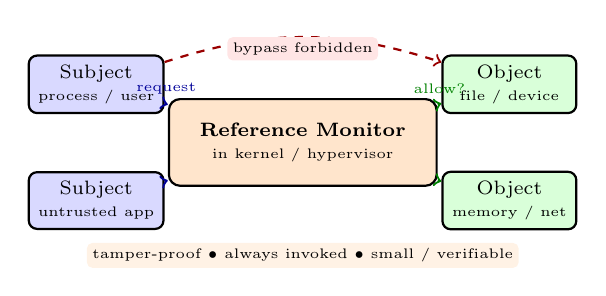
\begin{tikzpicture}[scale=0.82, every node/.style={font=\scriptsize},
  subj/.style={draw,thick,rounded corners=3pt,fill=blue!15,minimum width=1.7cm,minimum height=0.7cm,align=center},
  obj/.style={draw,thick,rounded corners=3pt,fill=green!15,minimum width=1.7cm,minimum height=0.7cm,align=center},
  rm/.style={draw,thick,rounded corners=4pt,fill=orange!20,minimum width=3.4cm,minimum height=1.1cm,align=center}]
\node[subj] (s1) at (-3.2,1.2) {Subject\\{\tiny process / user}};
\node[subj] (s2) at (-3.2,-0.6) {Subject\\{\tiny untrusted app}};
\node[obj] (o1) at (3.2,1.2) {Object\\{\tiny file / device}};
\node[obj] (o2) at (3.2,-0.6) {Object\\{\tiny memory / net}};
\node[rm] (rm) at (0,0.3) {\textbf{Reference Monitor}\\{\tiny in kernel / hypervisor}};
\draw[->,thick,blue!60!black] (s1) -- (rm) node[midway,above,font=\tiny] {request};
\draw[->,thick,blue!60!black] (s2) -- (rm);
\draw[->,thick,green!50!black] (rm) -- (o1) node[midway,above,font=\tiny] {allow?};
\draw[->,thick,green!50!black] (rm) -- (o2);
\draw[->,thick,red!60!black,dashed] (s1) to[bend left=18] (o1);
\node[font=\tiny,fill=red!10,rounded corners=2pt,inner sep=2pt] at (0,1.75) {bypass forbidden};
\node[font=\tiny,fill=orange!10,rounded corners=2pt,inner sep=2pt] at (0,-1.45) {tamper-proof $\bullet$ always invoked $\bullet$ small / verifiable};
\end{tikzpicture}
\caption{The reference monitor: every subject-to-object access is forced through a single, tamper-proof mediator. Dashed bypass must not exist.}
\label{fig:ref-monitor}
\end{figure}
% ============================================================
\section{The Reference Monitor and Complete Mediation}
\label{sec:ref-monitor}
Anderson (1972) defined the \emph{reference monitor} as an abstract machine that mediates all accesses. Three properties are non-negotiable:
\begin{definition}[Reference monitor properties]
A reference monitor must be (i)~\emph{always invoked} (complete mediation), (ii)~\emph{tamper-proof} (itself protected from modification), and (iii)~\emph{small enough to be verifiable} (amenable to analysis and testing).
\end{definition}
In practice the kernel's system-call path, the MMU/page tables, and the file-permission checks together implement the monitor. Hardware helps: CPU rings or privilege levels trap user-mode accesses; the kernel runs at higher privilege. Extended page tables and IOMMUs extend mediation to DMA from devices.
\begin{example}[Bypassing mediation]
A classic flaw: the OS checks \texttt{open("/safe/file")} but the actual read uses a file descriptor that an attacker swapped via a symlink (\texttt{TOCTOU}). The check and the use did not go through the same mediated path---property~(i) violated. Fix: check and open atomically, or operate on file descriptors already obtained via the mediator.
\end{example}
Verification matters: seL4 is a microkernel with a machine-checked proof that its access-control enforcement satisfies the reference-monitor properties; larger monolithic kernels trade verifiability for performance and rely on code review, fuzzing, and privilege minimisation instead.
\begin{remark}[Reference monitor vs.\ policy]
The monitor is the \emph{mechanism} that enforces; the \emph{policy} (Bell--LaPadula for confidentiality, Biba for integrity, RBAC/ABAC rules) is what it enforces. Confusing the two leads to monitors that correctly enforce the wrong policy.
\end{remark}
% ============================================================
\section{Privilege Separation}
\label{sec:priv-sep}
\emph{Privilege separation} splits a program into compartments with different privilege levels so that a compromise of the less-trusted part does not yield full privileges.
Think of a bank: the teller handles cash behind glass, but only the vault manager holds the vault key, and only for seconds.
\begin{definition}[Privilege bracketing]
Raise privilege, perform the minimal privileged operation, then drop privilege again. Never hold ambient authority while parsing untrusted input.
\end{definition}
\begin{lstlisting}[language=C]
// privilege bracketing (pseudo-C, POSIX)
uid_t real = getuid(), eff = geteuid();
seteuid(real);                 // drop to unprivileged
parse_untrusted_input(buf);    // bug here -> attacker gains only real uid
seteuid(eff);                  // re-acquire briefly
int fd = open("/var/log/auth", O_APPEND);
seteuid(real);                 // drop again immediately
write(fd, entry, len);
\end{lstlisting}
Other incarnations: OpenSSH splits \texttt{sshd} into a privileged monitor and an unprivileged slave communicating over a narrow IPC channel---even a full compromise of the pre-auth slave does not yield root. Chrome renders each tab in a low-privilege process; the browser process (broker) handles file and network access on its behalf.
Linux capabilities refine this further by breaking root into fine-grained units (\texttt{CAP\_NET\_BIND}, \texttt{CAP\_SYS\_ADMIN}, \texttt{CAP\_DAC\_OVERRIDE}) so a process need not be fully root. Dropping capabilities with \texttt{cap\_set\_proc} and retaining only the needed one is least privilege in action.
\begin{example}[setuid considered harmful]
A file owned by root with the setuid bit executes with the owner's privilege regardless of who launches it. A bug in a setuid helper (\texttt{/usr/bin/passwd}, \texttt{ping}) yields immediate privilege escalation. Modern systems minimise setuid binaries and prefer capabilities or a dedicated privileged daemon that validates requests.
\end{example}
% --- TikZ 2: Privilege separation / sandbox layers ---
\begin{figure}[h]
\centering
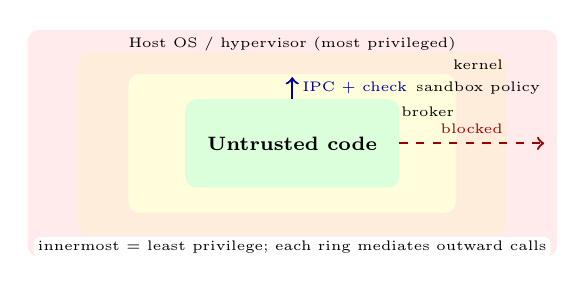
\begin{tikzpicture}[scale=0.80, every node/.style={font=\scriptsize}]
\fill[red!8,rounded corners=4pt] (-4.2,-1.8) rectangle (4.2,1.8);
\fill[orange!14,rounded corners=4pt] (-3.4,-1.45) rectangle (3.4,1.45);
\fill[yellow!14,rounded corners=4pt] (-2.6,-1.10) rectangle (2.6,1.10);
\fill[green!14,rounded corners=4pt] (-1.7,-0.70) rectangle (1.7,0.70);
\node at (0,0) {\textbf{Untrusted code}};
\node[font=\tiny,align=center] at (0,1.58) {Host OS / hypervisor (most privileged)};
\node[font=\tiny,align=center] at (2.95,1.25) {kernel};
\node[font=\tiny,align=center] at (2.95,0.88) {sandbox policy};
\node[font=\tiny,align=center] at (2.15,0.50) {broker};
\draw[->,thick,blue!60!black] (0,0.70) -- (0,1.05) node[midway,right,font=\tiny] {IPC + check};
\draw[->,thick,red!60!black,dashed] (1.7,0) -- (4.0,0) node[midway,above,font=\tiny] {blocked};
\node[font=\tiny,fill=white,rounded corners=2pt,inner sep=1.5pt] at (0,-1.65) {innermost = least privilege; each ring mediates outward calls};
\end{tikzpicture}
\caption{Layered privilege separation: untrusted code runs innermost; every sensitive operation must pass outward through broker and policy.}
\label{fig:priv-layers}
\end{figure}
% ============================================================
\section{Sandboxing}
\label{sec:sandbox}
A \emph{sandbox} is a tightly confined execution environment that restricts what the code inside can do even if it is malicious or buggy. Kernel-enforced sandboxes and user-mode sandboxes complement each other.
\paragraph{System-call filtering.} Linux \texttt{seccomp-bpf} lets a process install a BPF filter: only whitelisted syscalls proceed; others are killed or return an error. Firefox and Chrome use it to deny \texttt{execve}, \texttt{ptrace}, raw sockets to their renderers. OpenBSD \texttt{pledge} and \texttt{unveil} let a program voluntarily promise ``I will only need stdio and rpath''; the kernel kills it if it breaks the promise. The call \texttt{pledge("stdio rpath", NULL)} is a one-liner that enforces least privilege with almost no code.
\paragraph{Capability and policy sandboxes.} Capsicum (FreeBSD), Android app sandboxes (each app is a distinct UID with SELinux policy), and iOS entitlements restrict by capability tokens rather than ambient identity. Language-based sandboxes (WebAssembly, Java SecurityManager historically, browser JS) confine at the language runtime and complement OS sandboxes for defence-in-depth.
\begin{lstlisting}[language=Python]
# seccomp-style allowlist (conceptual Python)
ALLOWED = {"read", "write", "exit", "sigreturn"}
def syscall_filter(name, args):
    if name not in ALLOWED:
        raise SandboxViolation(f"syscall {name} denied by policy")
    return do_syscall(name, args)  # mediated path
# After installing filter, even compromised parser cannot execve("/bin/sh")
\end{lstlisting}
Two design rules matter. First, sandbox \emph{before} parsing untrusted bytes, not after---otherwise the attacker already ran code with ambient privilege. Second, keep the broker (the privileged process that serves sandbox requests) as small as possible; it is the new reference monitor and its bugs become sandbox escapes. Chrome's broker validates every \texttt{open} request against a policy table before forwarding it to the OS.
% ============================================================
\section{Virtualization and Container Security}
\label{sec:virt-containers}
\emph{Virtualization} runs multiple guest OSes on one host via a \emph{hypervisor}. Type~1 (bare-metal: Xen, Hyper-V, KVM as module) runs directly on hardware; Type~2 (hosted: VirtualBox, VMware Workstation) runs atop a host OS. Hardware extensions (Intel VT-x, AMD-V, EPT/NPT for nested paging, IOMMU/VT-d for device DMA) make traps and memory virtualisation efficient.
\emph{Containers} (Docker, LXC, Kubernetes pods) share the host kernel but isolate via OS mechanisms: \emph{namespaces} (PID, net, mount, UTS, user, IPC give each container its own view) and \emph{cgroups} (limit CPU, memory, I/O), plus \emph{seccomp}, AppArmor/SELinux, and dropped capabilities.
\begin{figure}[h]
\centering
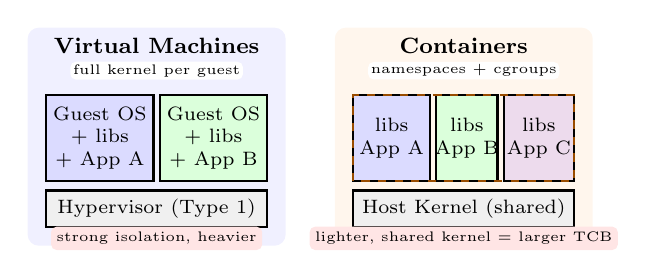
\begin{tikzpicture}[scale=0.78, every node/.style={font=\scriptsize}]
% VM side
\fill[blue!6,rounded corners=4pt] (-4.6,-1.9) rectangle (-0.4,1.65);
\node[font=\footnotesize\bfseries] at (-2.5,1.35) {Virtual Machines};
\draw[thick,fill=gray!12] (-4.3,-1.6) rectangle (-0.7,-1.0) node[midway] {Hypervisor (Type~1)};
\draw[thick,fill=blue!14] (-4.3,-0.85) rectangle (-2.55,0.55) node[midway,align=center] {Guest OS\\+ libs\\+ App A};
\draw[thick,fill=green!14] (-2.45,-0.85) rectangle (-0.7,0.55) node[midway,align=center] {Guest OS\\+ libs\\+ App B};
\node[font=\tiny,fill=white,rounded corners=2pt,inner sep=1pt] at (-2.5,0.95) {full kernel per guest};
% Container side
\fill[orange!7,rounded corners=4pt] (0.4,-1.9) rectangle (4.6,1.65);
\node[font=\footnotesize\bfseries] at (2.5,1.35) {Containers};
\draw[thick,fill=gray!12] (0.7,-1.6) rectangle (4.3,-1.0) node[midway] {Host Kernel (shared)};
\draw[thick,fill=blue!14] (0.7,-0.85) rectangle (1.95,0.55) node[midway,align=center] {libs\\App A};
\draw[thick,fill=green!14] (2.05,-0.85) rectangle (3.05,0.55) node[midway,align=center] {libs\\App B};
\draw[thick,fill=violet!14] (3.15,-0.85) rectangle (4.3,0.55) node[midway,align=center] {libs\\App C};
\draw[thick,dashed,orange!60!black] (0.7,-0.85) rectangle (4.3,0.55);
\node[font=\tiny,fill=white,rounded corners=2pt,inner sep=1pt] at (2.5,0.95) {namespaces + cgroups};
% vs label
\node[font=\tiny,align=center,fill=red!10,rounded corners=2pt,inner sep=2pt] at (-2.5,-1.78) {strong isolation, heavier};
\node[font=\tiny,align=center,fill=red!10,rounded corners=2pt,inner sep=2pt] at (2.5,-1.78) {lighter, shared kernel = larger TCB};
\end{tikzpicture}
\caption{VMs vs.\ containers: VMs virtualise hardware with a hypervisor and guest kernels; containers share one kernel and isolate with namespaces/cgroups.}
\label{fig:vm-vs-container}
\end{figure}
Threats differ: a \emph{VM escape} exploits a hypervisor bug (e.g.\ VENOM/QEMU floppy, CVE-2015-3456) to break into the host; a compromised guest that controls DMA without IOMMU can also attack host memory. Container escapes exploit kernel bugs or misconfiguration---privileged container, mounted Docker socket, \texttt{--privileged}, host-PID namespace, kernel CVE such as Dirty COW. Because containers share the kernel, a single kernel vulnerability breaks all containers on that host.
Hence hardening is essential: run containers rootless, with read-only filesystems (\texttt{--read-only}), no \texttt{CAP\_SYS\_ADMIN}, user namespaces remapping container root to an unprivileged host UID, and seccomp/AppArmor profiles that deny dangerous syscalls. For stronger isolation, gVisor inserts a user-space kernel (Sentry) that interposes syscalls, and Kata Containers wraps each container in a lightweight VM---trading some density for a hardware-enforced boundary. Choose VMs when tenants are mutually untrusted; choose containers when density and startup time dominate and the kernel TCB is acceptable.
% ============================================================
\section{Putting It Together: Hardening Checklist}
\label{sec:hardening-checklist}
A checklist ties the chapter together. Before shipping a service that handles untrusted input:
\begin{itemize}[leftmargin=*, itemsep=0.35em]
    \item \textbf{Enumerate trust boundaries.} What crosses from untrusted to trusted (file parses, IPC, device DMA)? Each crossing needs mediation.
    \item \textbf{Apply least privilege end-to-end.} Drop capabilities, use user namespaces, run renderers/workers as dedicated UIDs with no shell.
    \item \textbf{Sandbox before parse.} Instal seccomp/pledge \emph{before} the first byte of untrusted data is touched; verify the filter with \texttt{strace -c}.
    \item \textbf{Minimise broker TCB.} The broker that serves sandbox requests should validate, canonicalise, and log---no parsing of complex formats inside it.
    \item \textbf{Choose the right boundary.} Multi-tenant untrusted code $\to$ VMs or Kata/gVisor; single-tenant microservices $\to$ containers with tight seccomp/AppArmor.
    \item \textbf{Plan for escape detection.} Monitor for anomalous syscalls, unexpected capability use, and hypervisor/container CVEs; have a patch and live-migration story.
\end{itemize}
\begin{example}[Hardening a document converter]
A service converts uploaded PDFs to images. Bad design: a monolithic root process calls \texttt{libpoppler} on the upload. Good design: an unprivileged worker in a seccomp + mount-namespace sandbox with no network, read-only rootfs, and a tiny broker that only allows \texttt{open} of the single input file and \texttt{write} of the output. Even a full RCE in libpoppler yields only a sandboxed UID that cannot exec or exfiltrate.
\end{example}
\begin{remark}[Common pitfalls]
Overly broad seccomp allowlists (allowing \texttt{ptrace} or \texttt{mount}), writable \texttt{/proc} or Docker socket mounts, and retaining \texttt{CAP\_SYS\_ADMIN} ``just in case'' are the three most common sources of container escapes seen in CTFs and incident reports.
\end{remark}
\begin{example}[Why small TCB matters]
The classic qmail SMTP server (Bernstein) was split into mutually untrusting modules so that the parser that speaks to the network never runs as root. Despite decades of exposure, no remote root hole has been found---splitting and minimising the privileged part paid off. The same lesson drives seL4, gVisor's Sentry, and Chrome's broker: bugs are inevitable, but their location determines impact.
\end{example}
\begin{theorem}[Isolation reduces blast radius]
If compartment $C_1$ is compromised but $C_1$ holds no capability for object $O$ in $C_2$ and every path to $O$ is mediated, then $C_1$ cannot directly violate $C_2$'s integrity or confidentiality except via covert or side channels outside the modeled mediator.
\end{theorem}
In practice side channels (Spectre, Meltdown, cache timing) complicate the picture, which is why hardware isolation (page tables, EPT, IOMMU) must be combined with software hardening and constant-time handling of secrets.
% ============================================================
\section{Exercises}
\label{sec:ch07-exercises}
\begin{enumerate}[label=E7.\arabic*, leftmargin=*, itemsep=0.6em]
    \item \textbf{Reference monitor audit.} Your OS checks permissions on \texttt{open()} but a background thread can replace the pathname with a symlink between check and use (TOCTOU). Which reference-monitor property fails? Propose a fix using file descriptors or \texttt{openat2(RESOLVE\_NO\_SYMLINKS)} and argue why it restores the property.
    \item \textbf{Privilege bracketing.} A server parses a JPEG while holding \texttt{CAP\_SYS\_ADMIN}, then writes the log. Sketch an exploit if the parser has a buffer overflow. Rewrite the flow with bracketing/passing to a helper and explain why the blast radius shrinks.
    \item \textbf{seccomp policy design.} A PDF renderer needs \texttt{read}, \texttt{write}, \texttt{mmap}, \texttt{exit} but not \texttt{execve} or \texttt{socket}. Write a seccomp-bpf allowlist and describe what happens if the renderer is compromised and tries \texttt{execve("/bin/sh",\dots)}. What must the broker do for legitimate file-open requests?
    \item \textbf{VM vs.\ container trade-off.} You must run 100 mutually untrusted customer workloads on one host. Compare (a)~one VM per customer vs.~(b)~one container per customer on (i) isolation strength, (ii) memory/CPU overhead, (iii) patching burden. When would you choose Kata Containers/gVisor and why?
    \item \textbf{Container escape via misconfiguration.} A container is started with \texttt{docker run --privileged -v /:/host ubuntu bash}. Explain step-by-step how an attacker inside the container obtains host root. List three hardening flags that would block this path.
\end{enumerate}
% ============================================================
\section*{Chapter Notes}
Reference monitor and Anderson report (1972); Bell--LaPadula/Biba as policy models for the monitor. Least privilege (Saltzer \& Schroeder 1975). Privilege separation in OpenSSH (Provos et al.\ 2003), Chrome site isolation and sandbox (Reis \& Gribble). seccomp-bpf (Drewry 2012), OpenBSD \texttt{pledge}/\texttt{unveil}, Capsicum, seL4 verified kernel (Klein et al.\ 2009). Virtualization: Popek \& Goldberg (1974) requirements, Intel VT-x/AMD-V, EPT/NPT, IOMMU/VT-d. Containers: namespaces/cgroups, Docker, Kubernetes; hardening via rootless, gVisor (user-space kernel), Kata Containers (lightweight VMs). For a deeper view of capability systems see Capsicum (Watson et al.) and Fuchsia's capability-based security model.
% End of Chapter 7
